\documentclass[usenames,dvipsnames,8pt,aspectratio=169]{beamer}
\usepackage{amsmath,amsfonts,amssymb}
\usepackage{mathtools}
\usepackage{etex} %for Windows
\usepackage[utf8]{inputenc}
\usepackage[english, russian]{babel} 

%\usepackage{microtype}			% Better interword spacing and additional kerning.
\usepackage{ellipsis}			% Adjusted space with \dots between two words.
\usepackage{graphicx}
\usepackage{pstricks}

\usepackage{xcolor}


\usepackage{changepage}

\usepackage{algorithm}
\usepackage{algpseudocode}
%\usepackage[]{algorithm2e}
%\usepackage{algorithmic}

%\usepackage{tcolorbox}

\addtobeamertemplate{footline}{%
	\setlength\unitlength{1ex}%
	\begin{picture}(0,0) 
	% \put{} defines the position of the frame
	\put(155,0){\makebox(0,0)[bl]{
			%
\includegraphics[scale=0.65]{white_square}
			%
\includegraphics[scale=0.65]{dark_square}
			
\includegraphics[scale=0.65]{grey_circle}
	}}%
	\end{picture}%
}{}

\usepackage{tikz}
\usetikzlibrary{tikzmark,calc}
\usetikzlibrary{positioning, backgrounds}
\usetikzlibrary{arrows, chains, matrix, scopes, patterns, shapes, fit}
\usetikzlibrary{mindmap,trees,shadows}
\usetikzlibrary{decorations.pathreplacing}

\usepackage{pgfplots}

\pgfmathdeclarefunction{gauss}{2}{%
	\pgfmathparse{1/(#2*sqrt(2*pi))*exp(-((x-#1)^2)/(2*#2^2))}%
}


\tikzset{
	invisible/.style={opacity=0},
	visible on/.style={alt={#1{}{invisible}}},
	alt/.code args={<#1>#2#3}{%
		\alt<#1>{\pgfkeysalso{#2}}{\pgfkeysalso{#3}} % \pgfkeysalso doesn't change the path
	},
}

\newcommand\strikeout[2][]{%
	\begin{tabular}[b]{@{}c@{}} 
		\makebox(0,0)[cb]{{#1}} \\[-0.2\normalbaselineskip]
		\rlap{\color{Orange}\rule[0.5ex]{\widthof{#2}}{1.5pt}}#2
\end{tabular}}

\newcommand\Fontvi{\fontsize{11}{13.2}\selectfont}

\usepackage{listings} % for C++ code

\usepackage{braket}
%\usepackage[braket, qm]{qcircuit}



\usepackage[T1]{fontenc}
%\usepackage[sfdefault,scaled=.85]{FiraSans}
%\usepackage{newtxsf}
%\usepackage[nomap]{FiraMono}



%\renewtheorem{theorem}{Теорема}
%\renewtheorem{lemma}{Лемма}
%\renewtheorem{definition}{Определение}
%\renewtheorem{corollary}{Следствие}
%\renewtheorem{fact}{Факт}

\usefonttheme[onlymath]{serif}
\renewcommand\sfdefault{cmbr}

\renewcommand{\bfdefault}{sb}

\definecolor{CharCoalDark}{RGB}{13, 16, 19}
\definecolor{Orange}{RGB}{255, 165,0}
\definecolor{DarkOrange}{RGB}{255, 165,0}
\definecolor{LightSalmon}{RGB}{255, 160, 122}
\definecolor{LeafGreen}{RGB}{34, 139,  34}
\definecolor{Coral}{RGB}{255, 127, 80}
\definecolor{DarkTurquoise}{RGB}{0, 206, 209}

\definecolor{darkslateblue}{RGB}{72,61,139}

%\newtheorem{defRus}{Определение}
%\newtheorem{thmRus}{Теорема}
%s\newtheorem{corRus}{Следствие}

\def\darktheme{}
\ifdefined\darktheme
	\setbeamercolor{background canvas}{bg=CharCoalDark}
	\setbeamerfont{title}{series=\bfseries}
	\setbeamercolor{title}{fg=Orange}
	\setbeamercolor{section in toc}{fg=white}
	\setbeamercolor{frametitle}{fg=Orange}
	\setbeamercolor{normal text}{fg=white}
	%\setbeamercolor{normal text}{fontsize=12pt}
	\setbeamercolor{itemize item}{fg=Orange}
	\setbeamercolor{itemize item item}{fg=Orange}
	\setbeamercolor{enumerate item}{fg=Orange}
	\setbeamercolor{block title}{bg=DarkOrange,fg=white}
	\setbeamerfont{block title}{series=\bfseries}
	
	\setbeamertemplate{itemize item}[circle]
	%\setbeamertemplate{itemize subitem}[$\checkmark$]
	\setbeamertemplate{itemize subitem}{\color{Orange}\Large$\textbullet$}
	\setbeamertemplate{itemize subitem}{\color{Orange} \tiny $\blacksquare$}
\else
	\setbeamercolor{background canvas}{bg=white}
	\setbeamerfont{title}{series=\bfseries}
	\setbeamercolor{title}{fg=darkslateblue}
	\setbeamercolor{section in toc}{fg=black}
	\setbeamercolor{frametitle}{fg=darkslateblue}
	\setbeamercolor{normal text}{fg=black}
	%\setbeamercolor{normal text}{fontsize=9pt}
	\setbeamercolor{itemize item}{fg=darkslateblue}
	\setbeamercolor{itemize item item}{fg=darkslateblue}
	\setbeamercolor{enumerate item}{fg=darkslateblue}
	\setbeamercolor{block title}{bg=darkslateblue,fg=white}
	\setbeamerfont{block title}{series=\bfseries}
	
	\setbeamertemplate{itemize item}[circle]
	%\setbeamertemplate{itemize subitem}[$\checkmark$]
	\setbeamertemplate{itemize subitem}{\color{blue}\Large$\textbullet$}
	\setbeamertemplate{itemize subitem}{\color{blue} \tiny $\blacksquare$}

\fi

% footnote without a marker
\newcommand\blfootnote[1]{%
	\begingroup
	\renewcommand\footnoterule{}
	\renewcommand\thefootnote{}\footnote{#1}%
	\addtocounter{footnote}{-1}%
	\endgroup
}

\newcommand*{\Scale}[2][4]{\scalebox{#1}{\ensuremath{#2}}}%

\newcommand\Item[1][]{%
	\ifx\relax#1\relax  \item \else \item[#1] \fi
	\abovedisplayskip=0pt\abovedisplayshortskip=0pt~\vspace*{-\baselineskip}}

\pgfdeclareradialshading{ring}{\pgfpoint{0cm}{0cm}}%
{rgb(0cm)=(1,1,1);
	rgb(0.7cm)=(1,1,1);
	rgb(0.719cm)=(1,1,1);
	rgb(0.72cm)=(0.975,0,0);
	rgb(0.9cm)=(1,1,1)}

\usepackage[absolute,overlay]{textpos} %to clip to a corner
\newcommand\FrameText[1]{%
	\begin{textblock*}{\paperwidth}(\textwidth-35pt, 10 pt)
		\raggedright #1\hspace{.5em}
\end{textblock*}}

\makeatletter
\let\save@measuring@true\measuring@true
\def\measuring@true{%
	\save@measuring@true
	\def\beamer@sortzero##1{\beamer@ifnextcharospec{\beamer@sortzeroread{##1}}{}}%
	\def\beamer@sortzeroread##1<##2>{}%
	\def\beamer@finalnospec{}%
}
\makeatother

\AtBeginSection[]
{
	\begin{frame}<beamer>
		\frametitle{Outline}
		\tableofcontents[currentsection]
	\end{frame}
}


%\institute{ENS Lyon}
\author{\\ [10pt]
}
\titlegraphic{
	
	%\includegraphics[width=2.5cm]{erc_logo_gray}\hspace*{2.5cm}~%
	%\includegraphics[width=4.0cm]{ens_logo_gray}
}
\title{Лекция №1 \\[10pt]
		Часть 4. Семантическая стойкость. }

\date{ Елена Киршанова \\  \textbf{Курс ``Основы криптографии''} \\  }


\setbeamertemplate{navigation symbols}{} %removes navigation

% proper highlightling of a code-snippet
\lstset{language=C++,
	keywordstyle=\color{magenta},
	stringstyle=\color{Goldenrod},
	commentstyle=\color{gray},
	breaklines=false,
	%morecomment=[l][\color{magenta}]{\#}
}

%\setlength{\parskip}{8pt}
% ==================================================================
% Definitions for this paper
% ==================================================================
\mathchardef\hyphen="2D

\usepackage{multirow}
\usepackage{multicol} % For multiple coloumn environments
%\usepackage{stmaryrd} % For set brackets
% \setlength{\columnsep}{15pt} % Defining the coloumn seperation
% \setlength{\columnseprule}{1pt} % Place a line between coloumns
% \newcommand{\tab}{\hspace*{2em}}

%subscripts

\newcommand*\SmallTextScript[2]{{\mathchoice{\displaystyle #2}
		{\textstyle #2}%dito
		{\scalebox{#1}{\ensuremath{\scriptstyle #2}}}%
		{\scalebox{#1}{\ensuremath{\scriptscriptstyle #2}}}%
}}


% ADVERSARIES AND SUCH
\newcommand*{\poly}{\ensuremath{\mathrm{poly}}}
\newcommand*{\eps}{\ensuremath{\varepsilon}}
\newcommand*{\alg}{\ensuremath{\mathcal{A}}}

% GROUPS/DISTRIBUTIONS/SETS/LISTS
\newcommand{\N}{{{\mathbb N}}}
\newcommand{\Z}{{{\mathbb Z}}}
\newcommand*{\IZ}{\ensuremath{\mathbb{Z}}}
\newcommand*{\IN}{\ensuremath{\mathbb{N}}}
\newcommand*{\IQ}{\ensuremath{\mathbb{Q}}}
\newcommand{\R}{{{\mathbb R}}}
\newcommand*{\IR}{{{\mathbb R}}}
\newcommand{\Zp}{\ints_p} % Integers modulo p
\newcommand{\Zq}{\ints_q} % Integers modulo q
\newcommand{\Zn}{\ints_N} % Integers modulo N
\newcommand{\F}{\ensuremath{\mathbb{F}}}
\newcommand{\CC}{\ensuremath{\mathbb{C}}}

\newcommand{\GF}{\ensuremath{\mathbb{F}_2}}
\newcommand{\GFn}{\ensuremath{\mathbb{F}^n_2}}

%%% ALGORITHMS/PROCEDURES %%%
\newcommand{\Dec}{\textsf{Dec}}
\newcommand{\Enc}{\textsf{Enc}}
\newcommand{\KeyGen}{\textsf{KeyGen}}
\newcommand{\Gen}{\textsf{Gen}}
\newcommand{\sk}{\textsf{sk}}
\newcommand{\pk}{\textsf{pk}}
\newcommand{\vk}{\textsf{vk}}
\newcommand{\mesS}{\ensuremath{\mathcal{M}}}
\newcommand{\keyS}{\ensuremath{\mathcal{K}}}
\newcommand{\cipS}{\ensuremath{\mathcal{C}}}
\newcommand{\tagS}{\ensuremath{\mathcal{T}}}
\newcommand{\mactag}{\textsf{tag}}
\newcommand{\Hash}{\ensuremath{\mathcal{H}}}
\newcommand{\EID}{\ensuremath{\mathtt{EphID}}}


\newcommand{\adv}{\ensuremath{\mathcal{A}}}

\newcommand{\LWE}{\mathsf{LWE}}
\newcommand{\DCP}{\mathsf{DCP}}
\newcommand{\EDCP}{\mathsf{EDCP}}
\newcommand{\UEDCP}{\mathsf{U \text{-} EDCP}}
\newcommand{\GEDCP}{\mathsf{G \text{-} EDCP}}



%% Landau and proba
\newcommand{\bigO}{\mathcal{O}}
\newcommand*{\OLandau}{\bigO}
\newcommand*{\WLandau}{\Omega}
\newcommand*{\xOLandau}{\widetilde{\OLandau}}
\newcommand*{\xWLandau}{\widetilde{\WLandau}}
\newcommand*{\TLandau}{\Theta}
\newcommand*{\xTLandau}{\widetilde{\TLandau}}
\newcommand{\smallo}{o} %technically, an omicron
\newcommand{\wLandau}{\omega}
\newcommand{\negl}{\mathrm{negl}}
\newcommand*\PROB\Pr 
\DeclareMathOperator*{\EXPECT}{\mathbb{E}}
\DeclareMathOperator*{\VARIANCE}{\mathbb{V}}
\DeclareMathOperator*{\LOGBIAS}{\mathbb{LB}}

\newcommand{\supp}{\ensuremath{\mathsf{sup}}}
\newcommand{\Distr}{\ensuremath{\mathcal{D}}}

% Lattices

% \newcommand{\coset}{\Lambda} % Lambda Lattice
% \newcommand{\cosetPerp}{\Lambda^{\bot}} % Lambda_Perp Lattice
% \newcommand{\gadget}{\textbf{G}} %Gaget matrix
% \newcommand{\mes}{\textbf{m}} %message vector
% \newcommand{\AMat}{\textbf{A}} %A matrices
% \newcommand{\BMat}{\textbf{B}} %B matrices
% \newcommand{\RMat}{\textbf{R}} %R matrices
% \newcommand{\HMat}{\textbf{H}} %H matrices
% \newcommand{\XMat}{\textbf{X}} %H matrices
% \newcommand{\mbar}{\bar{m}} %mBar dimension
% % \newcommand{\gauss}{\mathcal{D}} % gaussian distribution
% \newcommand{\Id}{\textbf{I}} % Identity matrix
% \newcommand{\er}{\textbf{e}} % gaussian distr. vectors
% % \newcommand{\cipher}{\textit{c}} % ciphertext
% \newcommand{\Olwe}{\mathcal{O}_{\textsf{LWE}}} %LWE oracle
% \newcommand{\OSample}{\mathcal{O}_{Sample}} %LWE oracle
% \newcommand{\SigmaB}{\boldsymbol{\Sigma}} %semi-deifinite matrix Sigma%
% % \newcommand{\mods}{\text{ mod}}


%Vectors and Matrices

\newcommand{\AMat}{\mathbf{A}} %A matrices
\newcommand{\BMat}{\mathbf{B}} %B matrices
\newcommand{\DMat}{\mathbf{D}} %Diagonal


\newcommand{\HMat}{\ensuremath{\mathbf{H}}}
\newcommand{\QMat}{\ensuremath{\mathbf{Q}}}
\newcommand{\Id}{\ensuremath{\mathbf{I}}}
\newcommand{\ZeroM}{\textbf{0}} % Zero matrix

\newcommand{\avec}{\ensuremath{\mathbf{a}}}
\newcommand{\bvec}{\ensuremath{\mathbf{b}}}
\newcommand{\cvec}{\ensuremath{\mathbf{c}}}
\newcommand{\evec}{\ensuremath{\mathbf{e}}}
\newcommand{\rvec}{\ensuremath{\mathbf{r}}}
\newcommand{\svec}{\ensuremath{\mathbf{s}}}
\newcommand{\tvec}{\ensuremath{\mathbf{t}}}
\newcommand{\vvec}{\ensuremath{\mathbf{v}}}
\newcommand{\zvec}{\ensuremath{\mathbf{z}}}
\newcommand{\xvec}{\ensuremath{\mathbf{x}}}
\newcommand{\yvec}{\ensuremath{\mathbf{y}}}
\newcommand{\uvec}{\ensuremath{\mathbf{u}}}
\newcommand{\zerovec}{\ensuremath{\mathbf{0}}}

\newcommand{\nth}{^{\mathrm{th}}}
\newcommand{\nd}{^{\mathrm{nd}}}

\newcommand{\RepMMT}{\ensuremath{\mathcal{R}_{\protect\SmallTextScript{0.70}{\texttt{MMT}}}}}
\newcommand{\RepBJMM}{\ensuremath{\mathcal{R}_{\protect\SmallTextScript{0.70}{\texttt{BJMM}}}}}
\newcommand{\XOR}{\ensuremath{\mathtt{3XOR}}}


% % % % % \newcommand{\mb}[1]{\mathbf{#1}} % does not compile otherwise
%%% Removed by Gotti; this is just asking to screw up with packages that (properly) define \mb (mathbold)

% \newcommand{\bL}{\|\bvec_1\|} % b1 length that appears way too often
% \newcommand{\dL}{\|\dvec_1\|} % b1 length that appears way too oftend

%Norms and Scalar products

\newcommand*\abs[1]{\left\lvert#1\right\rvert}
\newcommand*\norm[1]{\left\lVert#1\right\rVert}
\newcommand*\normalabs[1]{\lvert#1\rvert} 
\newcommand*\normalnorm[1]{\lVert#1\rVert}
\newcommand*\bignorm[1]{\bigl\lVert#1\bigr\rVert}
\newcommand*\bigabs[1]{\bigl\lvert#1\bigr\rvert}
\newcommand*\Bigabs[1]{\Bigl\lvert#1\Bigr\rvert}
\newcommand*{\ScProd}[2]{\ensuremath{\langle#1\mathbin{,}#2\rangle}} %Scalar Product
% \newcommand*{\ScProd}[2]{\ensuremath{\langle#1 \:{,}\:#2\rangle}} %Scalar Product
\newcommand*{\bigScProd}[2]{\ensuremath{\bigl\langle#1\mathbin{,}#2\bigr\rangle}} %Scalar Product
\newcommand*{\BigScProd}[2]{\ensuremath{\Bigl\langle#1\mathbin{,}#2\Bigr\rangle}} %Scalar Product
\newcommand{\dist}{\ensuremath{\text{dist}}}


%Some other math operators

\DeclareMathOperator{\Span}{Span} %span of vectors
\DeclareMathOperator{\vol}{\mathrm{vol}} %volume
\DeclareMathOperator{\LW}{LambertW} %Lambert W function
\DeclareMathOperator{\SD}{SD}
\DeclareMathOperator{\gradient}{grad}
\DeclareMathOperator{\TRACE}{Tr}
\newcommand*{\dDR}{\mathrm{d}} %de-Rham-Differential (the d in dx, dy, dz and so on)


%Lists
\renewcommand{\L}{\ensuremath{\mathcal{L}}}

\renewcommand{\P}{\ensuremath{\mathcal{P}}}

\newcommand*{\Lout}{\ensuremath{\L_{\mkern-0.5mu\protect\SmallTextScript{0.85}{\textup{out}}}}}
\newcommand*{\Sout}{\ensuremath{S_{\mkern-0.5mu\protect\SmallTextScript{0.85}{\textup{out}}}}}
\newcommand{\wt}{\ensuremath{\mathit{wt}}}


\newcommand*{\softO}{\widetilde{\bigO}}

\newcommand{\const}{\mathsf{c}} 


\newcommand{\transpose}{\mkern0.7mu^{\mathsf{ t}}}

%proper overline reduced by 1.5mu
\newcommand{\overbar}[1]{\mkern 1.5mu\overline{\mkern-1.5mu#1\mkern-1.5mu}\mkern 1.5mu}

\DeclareMathOperator{\erf}{erf} %error function
\DeclareMathOperator{\erfc}{erfc} %complementary error function
\newcommand{\Er}{\ensuremath{\mathrm{Er}}} %complementary error function


% LATTICES

\newcommand{\Lat}{\ensuremath{\mathcal{L}}}
\newcommand*{\Sphere}[1]{\ensuremath{\mathsf{S}^{#1}}}
%\DeclareMathOperator{\Conf}{Conf}
\newcommand{\Conf}{\mathcal{C}}

%Thick line for table
\setlength{\doublerulesep}{0pt}
\newcommand{\thickline}{\hline\hline\hline}


%circled text
\newcommand*\circled[1]{\tikz[baseline=(char.base)]{
    \node[shape=circle,draw,inner sep=0.3 pt] (char) {\scriptsize #1};}}


%Fix Algorithmicx package
\def\NoNumber#1{{\def\alglinenumber##1{}\State #1}\addtocounter{ALG@line}{-1}}

%For comments
\newcommand{\GColor}{ForestGreen}  %Damiens' color
\newcommand{\EColor}{MidnightBlue} %Elena's color

\newcommand*{\E}[1]{{\color{\EColor} #1} } 
\newcommand*{\G}[1]{{\color{\GColor} #1} } 

%Proper limit with the subscript underneath
% \newcommand{\Lim}[1]{\raisebox{0.5ex}{\scalebox{0.8}{$\displaystyle \lim_{#1}\;$}}}


%TIKZ dense dotted pattern

\pgfdeclarepatternformonly{my dots}{\pgfqpoint{-1pt}{-1pt}}{\pgfqpoint{2.0pt}{2.0pt}}{\pgfqpoint{2pt}{2pt}}%
{
	\pgfpathcircle{\pgfqpoint{0pt}{0pt}}{.35pt}
	\pgfpathcircle{\pgfqpoint{1pt}{1pt}}{.35pt}
	\pgfusepath{fill}
}


\tikzset{
	master/.style={
		execute at end picture={
			\coordinate (lower right) at (current bounding box.south east);
			\coordinate (upper left) at (current bounding box.north west);
		}
	},
	slave/.style={
		execute at end picture={
			\pgfresetboundingbox
			\path  (lower right)rectangle (upper left) ;
		}
	}
} %all defs
\begin{document}
	
\begin{frame}
	\titlepage
\end{frame}

\begin{frame}{Информационно-теоретическая vs.\ семантическая стойкость}
\LARGE

\begin{table}

\begin{tabular}{c p{0.6cm} c}
	\textbf{\color{Orange}OTP}  &  & \textbf{\color{Orange} Вычислительный шифр} \\[10pt]

	 {\color{Orange}любые } атакующие &  &  {\color{Orange}вычилительно ограниченные } атакующие \\[10pt]
	 
	 Большие ключи $|\keyS| = |\mesS|$ &  & несколько сотен бит \\[10pt]
	 
	 Фиксированная длина $m$  &  &Любая длина $m$
	
\end{tabular}
\end{table}

\end{frame}

\begin{frame}{Семантическая безопасность: формальное определение}

\Large
\begin{center}
$
	\Pi = (\KeyGen, \Enc, \Dec)
$
\end{center}
\vspace{10pt}
%\centering
\begin{columns}
\begin{column}{0.7\textwidth}
\begin{tabular}{c c c}
	{\color{Orange} Челленджер $\mathcal{C}$ } & & {\color{Orange} Атакующий $\mathcal{A}$ }\\ [5pt]
	$k \leftarrow \KeyGen(1^\lambda)$ & $\xrightarrow{\quad \Huge \lambda \quad}$  &\\[5pt]
	 & $\xleftarrow{\; \Huge m_0, m_1 \in \mesS \;}$  &$m_0, m_1 \leftarrow \mesS $\\ [5pt]
	 $b \xleftarrow{\$} \{0,1\}  $& &\\ [5pt]
	 $c \leftarrow \Enc(k, m_b)$ & &\\ [5pt]
	 & $\xrightarrow{\quad c \quad}$ & \\ [5pt]
	 & $\xleftarrow{\quad \hat{b} \quad}$ & \\ [5pt]
\end{tabular}
	\begin{tikzpicture}[overlay]
		\draw[fill=none, draw=white, opacity=0.5] (-8.5,-2.3) rectangle (-5.3,3.0); 
		\draw[fill=none, draw=white, opacity=0.5] (-3.0,-2.3) rectangle (0.0,3.0); 
	\end{tikzpicture}
\end{column}
\begin{column}{0.35\textwidth}
	
\vspace{-60pt}
\hspace{-40pt}	$\mathtt{W_{\Pi, \adv}}$ -- событие $b == \hat{b}$. \\ [8pt]
\hspace{-40pt}	$\mathtt{SSAdv} = \abs{\Pr[\mathtt{W_{\Pi, \adv}}] - \frac{1}{2}}$ -выигрыш  $\adv$ \\ [5pt]
\end{column}
\end{columns}
\vspace{10pt}
	\color{Orange} Схема $\Pi$ --семантически безопасна, если для любого ppt $\adv:$  \[\mathtt{SSAdv} = \negl(\lambda).\] 
\end{frame}

\begin{frame}{Семантическая безопасность OTP}

\Large 
{\color{Orange} Теорема.}
	Для абсолютно стойкой схемы (OTP) и для всех атакующих $\adv$ выполняется 
	\[
		\Pr[\mathtt{W_{\Pi, \adv}}] = \frac{1}{2}.
	\]
	Эквивалентно
	\[
		\mathtt{SSAdv} = \abs{\Pr[\mathtt{W_{\Pi, \adv}}] - 1/2} = 0.
	\]
	
	
	\vspace{30pt}
	``Взлом'' абсолютно стойкой схемы эквивалентен угадываю ключа.
\end{frame}

\begin{frame}{Следствия семантической безопасности}
	\Large
	
	{\color{Orange} Теорема.} 
	
	$ \Pi = (\KeyGen, \Enc, \Dec) $ -- семантически стойкая схема. Тогда $\forall$ ppt $\adv$
	\[
	\Pr[\adv(\Enc(k, m)) \rightarrow m[i]] \leq \frac{1}{2} + \negl(\lambda) \qquad \forall i.
	\]
	
	\vspace{20pt}
	То есть семантически безопасная схема стойка к угадыванию $i$-ого бита открытого текста.
	
\end{frame}

\begin{frame}{Доказательство редукцией}
\Large
\vspace{-40pt}
\begin{align*}
		I_0 = \{m \in \mesS \; | \; m[i] = 0 \} \quad I_1 = \{m \in \mesS \; | \; m[i] = 1 \} \\
		\Pr[\adv(\Enc(k, m)) \rightarrow m[i]] \leq \frac{1}{2} + \negl(\lambda) 
\end{align*}
Построим $\adv'$, отличающий шифр-тексты $I_0$ от шифр-текстов $I_1$.

\vspace{10pt}

\begin{tabular}{c c c c c}
	{\color{Orange} $\mathcal{C}$ } & &  {\color{Orange} Атакующий $\mathcal{A'}$ } & & {\color{Orange} Атакующий $\mathcal{A}$ }  \\ [5pt]
	$k \leftarrow \KeyGen(1^\lambda)$ & $\xrightarrow{\quad  \lambda \quad}$ & & & \\
		& &		$m_0 \in I_0$&   &\\ [2pt]
		& $\xleftarrow{m_0, m_1}$ &		$m_1 \in I_1$&   &\\
		$b \xleftarrow{\$} \{0,1\}  $& & & &\\ 
		$c \leftarrow \Enc(k, m_b)$ & $\xrightarrow{\quad  c \quad}$ & $c$& $\xrightarrow{\lambda, c}$ &\\ 
		& $\xleftarrow{\quad\hat{b} \quad}$ & $\hat{b}: m[i]=m_{\hat{b}}[i]$ & $\xleftarrow{m[i]}$ & $m[i]$\\ [5pt]
\end{tabular}
\begin{tikzpicture}[overlay]
		\draw[fill=none, draw=white, opacity=0.5] (-12.3,-2.0) rectangle (-9.0,2.3); 
		\draw[fill=none, draw=white, opacity=0.5] (-7.5,-2.0) rectangle (-4.5,2.3); 
		\draw[fill=none, draw=white, opacity=0.5] (-3.3,-2.0) rectangle (-0.3,2.3); 
\end{tikzpicture}

\end{frame}


\begin{frame}{Доказательство редукцией}
\Large
\vspace{-40pt}
\begin{tabular}{c c c c c}
	{\color{Orange} $\mathcal{C}$ } & &  {\color{Orange} Атакующий $\mathcal{A'}$ } & & {\color{Orange} Атакующий $\mathcal{A}$ }  \\ [5pt]
	$k \leftarrow \KeyGen(1^\lambda)$ & $\xrightarrow{\quad  \lambda \quad}$ & & & \\
	& &		$m_0 \in I_0$&   &\\ [2pt]
	& $\xleftarrow{m_0, m_1}$ &		$m_1 \in I_1$&   &\\
	$b \xleftarrow{\$} \{0,1\}  $& & & &\\ 
	$c \leftarrow \Enc(k, m_b)$ & $\xrightarrow{\quad  c \quad}$ & $c$& $\xrightarrow{\lambda, c}$ &\\ 
	& $\xleftarrow{\quad \hat{b} \quad}$ & $\hat{b}: m[i]=m_{\hat{b}}[i]$ & $\xleftarrow{m[i]}$ & $m[i]$\\ [5pt]
\end{tabular}
\begin{tikzpicture}[overlay]
\draw[fill=none, draw=white, opacity=0.5] (-12.3,-2.0) rectangle (-9.0,2.3); 
\draw[fill=none, draw=white, opacity=0.5] (-7.5,-2.0) rectangle (-4.5,2.3); 
\draw[fill=none, draw=white, opacity=0.5] (-3.3,-2.0) rectangle (-0.3,2.3); 
\end{tikzpicture}

\end{frame}

\begin{frame}{Следствия семантической безопасности}
\Large
	{\color{Orange} Теорема.} 
	
	$ \Pi = (\KeyGen, \Enc, \Dec) $ -- семантически стойкая схема. Тогда $\forall$ ppt атакующего $\adv$ существует $\adv'$:
	\[
	| \Pr[\adv(\lambda, \Enc(k, m)) \rightarrow f(m)] - \Pr[\adv'(\lambda)\rightarrow f(m)] | \leq \negl(\lambda).
	\]
	
	\vspace{20pt}
	То есть семантически безопасная схема стойка к вычислению \emph{любой эффективной} функции $f(m)$.
\end{frame}

%\begin{frame}{Док-во через редукцию}
%	content...
%\end{frame}
%\begin{frame}{Pseudorandom Generators (PRGs)}
%\LARGE 
%	Idea: `Stretch' truly random $\ell$-bits seed $s$ into a longer $L$-bits `random looking' string  
%	\vspace{15pt}
%	Define
%	\LARGE
%	\begin{align*}
%		G : \{0,1\}^{\ell} & \rightarrow \{0,1\}^{L}:	\\
%		s & \mapsto G(s) 
%	\end{align*}
%	
%	{\color{Orange}\textbf{Intuition:}} an ppt adversary cannot tell the difference between $G(s)$ and $r \leftarrow \{0,1\}^L$.
%	
%\end{frame}
%\begin{frame}{Computational Security}
%\Large
%	{\color{Orange}\textbf{Perfect Secrecy}}
%	\begin{itemize}
%		\item Information-theoretic (strong) security against {\color{Orange}\textbf{unbounded}} adversary
%		\item Impractical key space size
%	\end{itemize}
%		\vspace{15pt}
%	{\color{Orange}\textbf{Computational Security}}
%	\begin{itemize}
%		\item We usually use keys of sizes $128, 256$ bits
%		\item Security against {\color{Orange}\textbf{ppt}} adversaries
%		\item Unbounded adversary with access to plaintext-ciphertext pairs $(m_i, c_i)$ can launch an exhaustive search for $k \in \keyS$ s.t.\ $\Enc(k, m_i) == c_i \; \forall i$.
%	\end{itemize}
%\end{frame}
%

%
%\begin{frame}{Statistical tests}
%\Large 
%A {\color{Orange}\textbf{Is $\Pi$ statistical test}} on $\{0,1\}^n$ is an algorithm $A$ s.t. $A(x)$ outputs $0$ (=``not random'') or $1$ (=``random'') \\[10pt]
%\LARGE
%\begin{enumerate}
%	\item $A(x) = 1 \quad \abs{\# 0(x) - \# 1(x)} \leq 10 \sqrt{n}$  \\ [10pt]
%	\item $A(x) = 1 \quad \abs{\# 00(x) - n/4} \leq 10 \sqrt{n}$  \\ [10pt]
%	\item $A(x) = 1 \quad \max \mathsf{len}\{1...1(x) \} \leq 10 \log n$  \\ [10pt]
%\end{enumerate}
%
%\end{frame}
%
%\begin{frame}{Secure PRG}
%\Large
%	\begin{block}{Formal definition}
%	A PRG $G$ is an efficient deterministic algorithm that given a seed $s \in \mathcal{S} = \{0,1\}^{\ell}$ outputs an $r \in \mathcal{R} = \{0,1\}^L$ 
%	
%\end{block}
%	{\color{Orange}\textbf{Attack game for PRG:}} \\
%	\vspace{15pt}
%	%For a given PRG $G$ and a given adversary $\mathcal{A}$, define 	{\color{Orange}\textbf{Experiment 0:}} and 	{\color{Orange}\textbf{Experiment 1:}}: \\
%	{\color{Orange}\textbf{Experiment 0:}}
%	The Challenger computes $r \in \mathcal{R}$ as
%	\begin{align*}
%		 \Huge	s &\leftarrow \mathcal{S} \\
%		 \Huge	r & \leftarrow G(s)
%	\end{align*}
%	\pause
%	{\color{Orange}\textbf{Experiment 1:}}
%	The Challenger computes $r \in \mathcal{R}$ as
%	\begin{align*}
%		 \Huge	r & \leftarrow \{0,1\}^{L}
%	\end{align*}
%	Let $W_b$ be the event that $\mathcal{A}$ outputs $b$. \\
%	 $\mathcal{A}$'s advantage: $	\mathsf{PRGadv} \left[  \mathcal{A}, G \right ] = |\Pr[W_0] - \Pr[W_1]|$. \\[5pt]
%	 
%	 A PRG $G$ is {\color{Orange}\textbf{secure}} if $	\mathsf{PRGadv}$ is negligible for all ppt $\mathcal{A}$.
%	 
%
%\end{frame}
%
%\begin{frame}{Stream Cipher = OTP with keys output by a PRG}
%\LARGE
%	Let $G: \{0,1\}^{\ell} \rightarrow \{0,1\}^L$ \\[5pt]
%	
%	The {\color{Orange}\textbf{stream cipher}} $\Pi = (\KeyGen, \Enc, \Dec)$ is defined over
%	\begin{itemize}
%		\item $\keyS = \{0,1\}^{\ell}$ \\
%		\item $\mesS = \{0,1\}^{L}$ \\
%		\item $\cipS = \{0,1\}^{L}$ \\
%	\end{itemize}
%	\vspace{10pt}
%	For $s \in \{0,1\}^{\ell}$
%	\begin{itemize}
%		\item $\Enc(s, m \in \{0,1\}^L): c = G(s) \oplus m$ \\[10pt]
%		\item $\Dec(s, c \in \{0,1\}^L): m = G(s)\oplus c$ \\
%	\end{itemize}
%
%\end{frame}
%
%\begin{frame}{Semantic Security}
%		\begin{tikzpicture}
%			\draw[-stealth, thick] (-1.8,-1.0) -- (-1.0,-1.0) node[above,midway]{\Huge $b$};
%			\draw[fill=CharCoalDark, draw=white, opacity=0.5] (-1.0,-2.0) rectangle (1.8,1.8)  node[color=white, opacity=1,align=center, pos=0.5]{
%				\Large  {\color{Orange}{\underline{Challenger}} }  \\[18pt]
%				\Huge $k \leftarrow \keyS$
%			};
%			\draw[stealth-, thick] (1.8,0.5) -- (6.5,0.5) node[above,midway]{\Large $m_0, m_1 \in \mesS,  |m_0|=|m_1|$};
%			\draw[-stealth, thick] (1.8,-0.5) -- (6.5,-0.5) node[above,midway]{\Large $c \leftarrow \Enc(k,m)$};
%			\draw[fill=CharCoalDark, draw=white, opacity=0.5] (6.5,-2.0) rectangle (8.0,1.8)  node[color=white,pos=0.8] {
%				\Large  {\color{Orange}{\underline{$\mathcal{A}$}} }
%			};
%			\draw[-stealth, thick] (8.0,-1.0) -- (9.0,-1.0) node[above,midway]{\Huge $b'$};
%		\end{tikzpicture}
%		\Large
%		\vspace{15pt} \\
%		\centering
%		
%		Let $W_b$ be the event that $\mathcal{A}$ outputs $b$. \\
%		$\mathcal{A}$'s advantage: $	\mathsf{Adv} \left[  \mathcal{A}, \Enc \right ] = |\Pr[W_0] - \Pr[W_1]|$. \\[5pt]
%		
%		 $\Pi$ is {\color{Orange}\textbf{semantically secure}} if $	\mathsf{PRGadv} = \negl(\lambda)$  for all ppt $\mathcal{A}$.
%\end{frame}
%
%%\begin{frame}{Unpredictability of a PRG}
%%	content...
%%\end{frame}
%
%\begin{frame}{Semantic Security of $\Pi$}
%\LARGE
%	\begin{theorem}
%		If $G$ is a secure PRG, then the stream cipher $\Pi$ constructed from $G$ is semantically secure.
%	\end{theorem}
%\vspace{20pt}
%{\color{Orange}\textbf{Proof strategy: }} for any adversary $\mathcal{A}$ against semantic security, $\exists$ an adversary $\mathcal{B}$ against $G$.
%\end{frame}
%
%\begin{frame}{QUESTION!}
%	\LARGE
%	
%	Let $G$ be a PRG that the last bit of the output is always 0. \\[10pt]
%	Let $\Pi$ be a stream cipher constructed from $G$.\\[15pt]
%	\centering
%	{\color{Orange}\textbf{Is $\Pi$ semantically secure?}} 
%\end{frame}
%
%
%
%\begin{frame}{Constrictions of a PRG: Salsa and ChaCha}
%\Large
%	\begin{itemize}
%		\item Salsa20,ChaCha20: proposed by D.Bernstein in 2005, 2008
%		\item used in many TLS cipher suits
%		\item Input: $256$-bit seed and a parameter $L$
%		\item Output: $(256 \cdot L)$-bit pseudorandom string
%	\end{itemize}
%	\vspace{20pt}
%	\pause
%	Two components
%	\begin{enumerate}
%		\item $\mathsf{pad}(s, j, 0)$: takes a seed $s$, a $64$-bit counter $j$ and a $64$-bit nonce\\
%		Output: $512$-bit block
%		\item a fixed public permutation $\pi: \{0,1\}^{512} \rightarrow \{0,1\}^{512}$
%	\end{enumerate}
%	\vspace{20pt}
%	See \url{https://cr.yp.to/chacha.html} for details
%\end{frame}
%
%\begin{frame}{ChaCha PRG}
%\begin{figure}
%	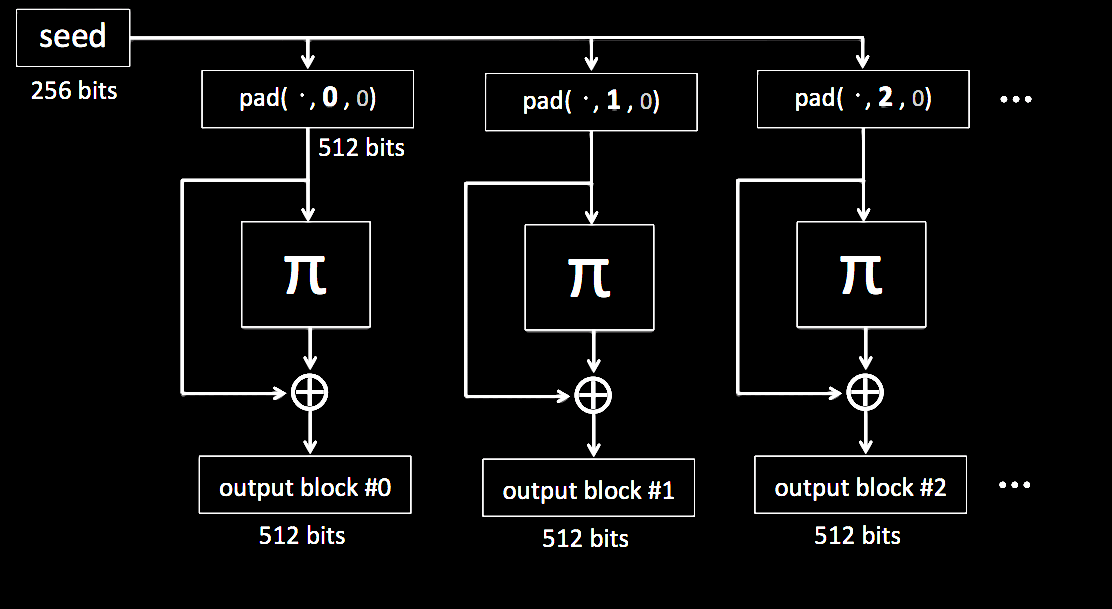
\includegraphics[width=\textwidth]{ChaCha20}
%\end{figure}
%
%Nonce -- the third parameter of $\mathsf{pad}(s, j, 0)$ is used to convert a PRG into a PRF (useful for encryption of multiple messages).
%\vfill
%\small
%{\color{gray}\textbf{picture is taken from D.Boneh, V.Shoup A Graduate Course in Applied Cryptography}} 
%\end{frame}
%
%\begin{frame}{(Somewhat) Broken PRGs}
%\LARGE
%\begin{enumerate}
%	\itemsep2em 
%	\item {\color{Orange}\textbf{linear congruential generators}} 
%	\begin{itemize}
%		\LARGE
%				\itemsep5pt  
%		\item had been used in glibc, Microsoft Visual Basic, Java
%		\item notorious for RANDU
%		\item \textbf{not cryptographically secure PRG!}
%	\end{itemize}
%
%	\item {\color{Orange}\textbf{RC4}} 
%	\begin{itemize}
%		\LARGE
%		\itemsep5pt 
%		\item proposed by R.Rivest  in 1987
%		\item used to be a part of TLS, 802.11b WEP
%		\item \textbf{not cryptographically secure PRG!}
%	\end{itemize}
%
%	\item {\color{Orange}\textbf{Linear feedback shift registers}}
%	\begin{itemize}
%			\LARGE
%			\itemsep5pt
%		\item used for protecting movies on DVD disks
%		\item weakly security  PRG (Trivium)
%	\end{itemize} 
%\end{enumerate}
%
%\end{frame}
%
%\begin{frame}{A Random Number Generator}
%	\Large
%	\begin{itemize}
%		\itemsep7pt
%		\item In practice, random bits are generated using a random number generator,  RNG
%		\item An RNG outputs a sequence of pseudorandom bits
%		\item Unlike PRG, an RNG take additional input (entropy source)
%		\item Example in Linux: $\mathsf{/dev/random}$
%		\item Entropy is usually taken from hardware (keyboard/mouse events, hardware interrupts, jitters).
%	\end{itemize}
%\end{frame}
%
%\begin{frame}{Application: Coin flipping}
%\LARGE
%Task:  throw a fair coin over without interaction 
%\begin{center}
%	\begin{tabular}{c c c c c}
%		 \multicolumn{5}{c}{$G: \{0,1\}^{\ell} \rightarrow \{0,1\}^{L}$}\\[10pt]
%		& Bob  & & Alice &  \\
%		 & \multirow{5}{*}{
\includegraphics[scale=0.20]{Bob}} & &
%		\multirow{5}{*}{
\includegraphics[scale=0.20]{Alice}} &  \\
%		&  &  & & $r \leftarrow \{0,1\}^{L}$  \\
%		&  & $\xleftarrow{r}$ & &  \\
%		Flips a coin &   & &  &  \\
%		$b \in \{0,1\}$&  & & &  \\
%		$s \in \{0,1\}^{\ell}$&  & & &  \\[15pt]
%		\multicolumn{5}{l}{$\mathsf{commit}(b, r, s)  = 
%			\begin{cases}
%			G(s), & b = 0\\
%			G(s) \oplus r, & b=1
%			\end{cases}
%			$}  \\
%		&  & $\xrightarrow{\mathsf{commit}(b, r, s)} $ & &  \\
%	\end{tabular}
%\end{center}
%
%\end{frame}

\end{document}